The measurement of current $I$ was shown in Table \ref{tab-deg-20}.
\begin{table}[!h]
\begin{center}
\begin{tabular}{|c|c|c||c|c|c|}
\hline
\multicolumn{6}{|c|}{Rotation angle of 1/4-wave plate: $20^\circ$}\\
\hline
\multicolumn{6}{|c|}{Maximum Electric Current $I_0$ $4.169\pm0.001$ [$\mu A$]}\\
\hline
$\theta$&$I[\mu A]\pm0.01[\mu A]$&$I/I_0$&$\theta$&$I[\mu A]\pm0.01[\mu A]$&$I/I_0$\\
\hline
$0^\circ$	&	3.641	&	$0.873\pm0.0003$	&	$180^\circ$	&	3.637	&	$0.872\pm0.0003$	\\
\hline
$10^\circ$	&	4.010	&	$0.962\pm0.0003$	&	$190^\circ$	&	4.001	&	$0.960\pm0.0003$	\\
\hline
$20^\circ$	&	4.163	&	$0.999\pm0.0003$	&	$200^\circ$	&	4.169	&	$1.000\pm0.0003$	\\
\hline
$30^\circ$	&	4.087	&	$0.980\pm0.0003$	&	$210^\circ$	&	4.103	&	$0.984\pm0.0003$	\\
\hline
$40^\circ$	&	3.797	&	$0.911\pm0.0003$	&	$220^\circ$	&	3.827	&	$0.918\pm0.0003$	\\
\hline
$50^\circ$	&	3.313	&	$0.795\pm0.0003$	&	$230^\circ$	&	3.551	&	$0.852\pm0.0003$	\\
\hline
$60^\circ$	&	2.700	&	$0.648\pm0.0003$	&	$240^\circ$	&	2.765	&	$0.663\pm0.0003$	\\
\hline
$70^\circ$	&	2.056	&	$0.493\pm0.0003$	&	$250^\circ$	&	2.108	&	$0.506\pm0.0003$	\\
\hline
$80^\circ$	&	1.433	&	$0.344\pm0.0003$	&	$260^\circ$	&	1.478	&	$0.355\pm0.0003$	\\
\hline
$90^\circ$	&	0.981	&	$0.235\pm0.0002$	&	$270^\circ$	&	0.953	&	$0.229\pm0.0002$	\\
\hline
$100^\circ$	&	0.626	&	$0.150\pm0.0002$	&	$280^\circ$	&	0.604	&	$0.145\pm0.0002$	\\
\hline
$110^\circ$	&	0.461	&	$0.111\pm0.0002$	&	$290^\circ$	&	0.452	&	$0.108\pm0.0002$	\\
\hline
$120^\circ$	&	0.518	&	$0.124\pm0.0002$	&	$300^\circ$	&	0.518	&	$0.124\pm0.0002$	\\
\hline
$130^\circ$	&	0.791	&	$0.190\pm0.0002$	&	$310^\circ$	&	0.801	&	$0.192\pm0.0002$	\\
\hline
$140^\circ$	&	1.261	&	$0.302\pm0.0003$	&	$320^\circ$	&	1.292	&	$0.310\pm0.0003$	\\
\hline
$150^\circ$	&	1.828	&	$0.438\pm0.0003$	&	$330^\circ$	&	1.854	&	$0.445\pm0.0003$	\\
\hline
$160^\circ$	&	2.482	&	$0.595\pm0.0003$	&	$340^\circ$	&	2.550	&	$0.612\pm0.0003$	\\
\hline
$170^\circ$	&	3.117	&	$0.748\pm0.0003$	&	$350^\circ$	&	3.142	&	$0.754\pm0.0003$	\\
\hline
\end{tabular}
\caption{Measurement data for the 1/4-wave plate (rotation angle $20^\circ$).}\label{tab-deg-20}
\end{center}
\end{table}

The relation between rotation angle and light intensity was plotted in Figure \ref{fig-deg-20}.
\begin{figure}[H]
\centering
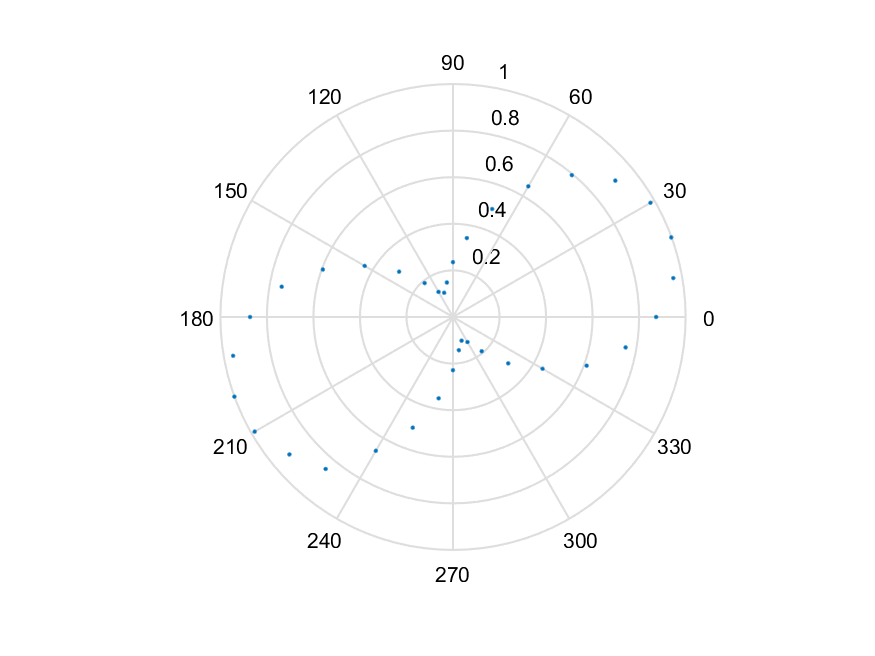
\includegraphics[scale=0.5]{deg-20.png}
\caption{$\theta$ vs. $I/I_0$ graph.}
\label{fig-deg-20}
\end{figure}
